\documentclass[journal]{IEEEtran}


\usepackage[czech]{babel}


% DOPLNIJICI BALICKY
\usepackage[utf8]		%	Kódování zdrojových souborů je Windows-1250
	{inputenc}					% Balíček pro nastavení kódování zdrojových souborů
\usepackage{cmap} 		% Balíček cmap zajišťuje, že PDF vytvořené `pdflatexem' je
											% plně "prohledávatelné" a "kopírovatelné"

\usepackage{amsmath}
\usepackage{caption}
\usepackage{dsfont}
\usepackage{layouts}
\usepackage{graphicx}
\usepackage{hyperref}
\usepackage{subcaption}
\usepackage{acro}

% zkratky
\DeclareAcronym{MSE}{
  short=MSE,
  long=mean squared error
}

\DeclareAcronym{PSNR}{
  short=PSNR,
  long=peak signal-to-noise ratio
}

\DeclareAcronym{SSIM}{
  short=SSIM,
  long=structural similarity
}

\DeclareAcronym{OCR}{
  short=OCR,
  long=Optical Character Recognition
}

\DeclareAcronym{IDE}{
  short=IDE,
  long=Integrated Development Environment
}

\DeclareAcronym{API}{
  short=API,
  long=Application Programming Interface
}


\usepackage[
style=numeric,
sorting=none
]{biblatex}
\addbibresource{literature.bib} %Import the bibliography file


\def\contentsname{Contents}
\def\listfigurename{List of Figures}
\def\listtablename{List of Tables}
\def\refname{References}
\def\indexname{Index}
\def\figurename{Obr.}
\def\tablename{Tab.}
\def\partname{Part}
\def\appendixname{Appendix}
\def\abstractname{Abstract}
% IEEE specific names
\def\IEEEkeywordsname{Klíčová slova}
\def\IEEEproofname{Proof}




\title{Smart Dictionary}


\author{Bc. Jiří Bönsch
        \linebreak
        Faculty of Informatics and Management
        \linebreak
        University of Hradec Kralove,
        \linebreak
        Hradec Kralove, Czech Republic
        \linebreak
        bonscji1@uhk.cz

}

\begin{document}

% make the title area
\maketitle

% As a general rule, do not put math, special symbols or citations
% in the abstract or keywords.
\begin{abstract}
        Tento článek se zabývá problematikou efektivity učení, specificky rozdíly mezi ručně psanými a digitálními poznámkami.
        Tato problematika často vzniká při studiu slovní zásoby cizího jazyka.
        Ručně psané poznámky si student lépe pamatuje, digitální poznámky jsou ale přístupnější a dovolují navíc využívání pomocných technik a moderní technologie.
        Tento článek navrhuje jako řešení digitalizaci ručně psané textu spojenou s využitím databáze pro ukládání učené látky.
        Bohužel se ukázalo, že volně dostupné prostředky pro digitalizaci nejsou zatím dostatečně vyspělé, aby bylo možné použít je tomuto účelu.
        Na závěr jsou ukázány porovnání 2 vybraných prostředků, Tesseract a EasyOCR, s testovacím komerčním řešením Pen to Print.
\end{abstract}

% Note that keywords are not normally used for peerreview papers.
\begin{IEEEkeywords}
Memory, Computer vision, Acquisition of knowledge, Educational psychology
\end{IEEEkeywords}


\IEEEpeerreviewmaketitle



\section{INTRODUCTION/ÚVOD}

\subsection{Úvod}
Současná doba je spojená s pokrokem technologie.
Nové poznatky a technologie prolínají každou část lidského života, není tomu jinak ani v rámci studia.
Elektronické pomůcky stále více nahrazují pomůcky klasické.
Tužka je nahrazena elektronickým perem.
Papír nahrazen tabletem.
Podobná nahrazení jsou ve všech aspektech studia, je však nutné si položit otázku.
Vede toto nahrazení k lepším studijním výsledkům?

\subsection{První studie}
Vědecké studie tuto skutečnost dlouhodobě zkoumají.
Existují velice jasné návaznosti, kdy novější studie upřesňuje výsledky starších studií, tuto studii doplňují o novější aplikace technologie.
Příkladem může být zaměření na psaní poznámek v akademické prostředí.\cite{mightier_pen}
Studie testuje, zda existuje významný rozdíl mezi zapisováním poznámek na notebooku oproti zapisování poznámek na papír pomocí pera.
Zkoumání vede k zajímavým výsledkům.
Psaní pomocí pera je pro cíl zapamatování studované látky efektivnější nežli zapisování poznámek na notebooku.
Hlavním důvodem je skutečnost, že psaní perem je pomalejší.
To vede k nutnosti zvolit informace, které student zapíše.
Notebook v tomto ohledu naopak dovoluje doslovné zapisování výkladu, kdy student nemusí již při psaní o studované látce více přemýšlet.
Zájem může vzbudit i dodatečný výzkum, zaměřený na seznámení uživatelů notebooků s nevýhodami této zapisovací strategie.
I když uživatelé znaly nevýhody, nevedlo to k významné změně strategie a výsledků.

\subsection{Druhá studie}
Velkou mezerou předchozí studie je existence digitálních per.
V původní studii jejichž dopad nebyl zkoumán, existuje však novější studie, která se zabývá právě touto problematikou.
Studie zkoumá, zda využívání klasických per, digitálních per nebo klávesnice vede k lepším výsledků při studiu jednotlivých slov.\cite{advantage_of_handwriting}
Ukazuje se, že i pro studování jednotlivých slov je stále nejlepším řešením psaní perem.
Zajímavé jsou zaznamenané rozdíly mezi perem digitálním a klasickým.
U zkoumaných subjektů, kteří mají zkušenosti s digitálním perem, nebyl zaznamenán značný rozdíl mezi typy pera.
Pouze u subjektů bez předchozích zkušeností se projevil statisticky významný rozdíl ve prospěch klasického pera.
Je možné, že rozdíly mezi typy pera u nezkušených uživatelů mohou být způsobené zvýšenou kognitivní zátěží způsobenou používáním nové studijní pomůcky.
Opět se potvrzuje fakt, že používání kteréhokoli pera bylo pro studium slov výrazně lepší než pouze zapisování s pomocí klávesnice.

\subsection{Třetí studie}
Předcházející sekce mohou vyvolávat dojem nevhodnosti technologie pro usnadnění studia dalších jazyků.
Základ tohoto dojmu je však postaven na velice specifické sféře mnohem složitějšího problému.
Jako řešení je možné využít studie zabývající se celkovou problematikou.
Meta-analýza zkoumající více jak 30 studií zkoumajících toto téma představuje rozsáhlejší pohled na problematiku studia více jazyků.\cite{technology_vocab} Analýza jasně ukazuje, že podpora studia využitím moderní technologie vedla k lepším výsledkům zkušebních testů.
Nezáleží ani, zda byl test psán okamžitě po studiu, nebo až s časovým odstupem.
Vždy je vidět jasná korelace lepších výsledků s používáním moderní technologie.
Obzvláště zajímavé poznatky však vynikly při komparaci výsledků věkových skupin a také typu využívané technologie.
Nejlepší výsledky přineslo využití moderních technologií u vysokoškolských studentů.
Nelze s jistotou říci, zda je tato skutečnost způsobena jejich schopností pracovat s moderními technologiemi nebo jejich znalostní bází anglického jazyka.
U předškoláků a na prvním stupni základních škol naopak využití moderních technologií nepřineslo značný přínos.
Analýza také ukazuje jasnou preference studia látky na mobilních telefonech.
Za pomoci mobilního telefonu je možné studovat kdekoli a to v porovnání se studiem na stolních počítačích ve třídě k vedlo k lepším výsledkům.

\subsection{Závěr studií}
Použití moderních technologií má zcela jasně smysl.
Nelze však bezmyšlenkovitě vynucovat jejich používání.
Můžeme uvažovat o nutnost zaměřit nasazování moderních technologií pouze do specifických odvětví studia.
Tento přístup by měl do budoucna vést ke zvýšení studijní efektivity.

\section{PROBLEM DEFINITION/ DEFINICE PROBLÉMU}

\subsection{Problematika}
Jak již bylo zmíněno, pro maximalizaci efektivity studia by bylo ideální využívat jak výhody zapisování materiálu perem, tak výhody digitální podoby materiálu. Pokud se podíváme blíže na úlohu studování slovní zásoby jazyka, můžeme jasně identifikovat tyto dva protilehlé faktory. Pro lepší zapamatování slov je lepší zapisovat je perem, naopak pro možnosti opakování a také dodatečných pomůcek v podobě optimalizace a preferování zaměření na složitá slova je ideální digitální forma. Cíl je jasný, najít nebo vytvořit řešení, která umožní využívat tyto dvě nekompatibilní metodologie současně.

\subsection{Průzkum existujících řešení}
Tato práce není první, která se danou problematikou zabývá.
Hlubší průzkum problematiky vede k již existujícím řešením v podobě digitalizace psaného textu.
Je možné nalézt hned několik možností, jak digitalizace dosáhnout.
Existence několika srovnatelných možností však poukazuje na fakt, že neexistuje jedno perfektní řešení, které by bylo jasně lepší nežli všechna ostatní a tak uživateli preferováno.
Ne každý postup je vhodný pro každého uživatele, ať už se jedná o problematiku ceny, požadavků na fyzická zařízení nebo dokonce přesnost převodu či osobní principy.\cite{aarp_digitalization, popupalr_science_digitalization_with_pens}

\paragraph{Smart pera}
Prvním možným řešením jsou systémy využívající Smart pera.
Tento systém má 3 části, již zmíněné Smart pero, speciální tečkovaný blok a aplikaci.
Smart pero je schopno klasicky zapisovat a při tomto zápisu snímá pohyby ruky, tečkovaný blok pak využívá k přesnému zaznamenávání umístění psaného textu na stránku. Všechna tato data jsou pak zaslána aplikaci, která vytváří přesnou digitální kopii psaného textu. Aplikace je také schopna ručně psanou digitální kopii převést do klasického formátu Microsoft Word. Hlavní výhodou tohoto řešení je značná přesnost, ne každý je však ochotný platit prémium za takto specifický use-case.\cite{popupalr_science_digitalization_with_pens}

\paragraph{Smartphone}
Dalším řešením je využívání smartphonu, který v dnešní době vlastní většina populace.
Apple od verze iOS 15 zabudoval do operačního systému aplikaci Live Text, která uživateli dovoluje zvolit a poté zvolený text vykopírovat.
Android  tuto funkcionalitu v operačním systému zabudovanou nemá. tuto skutečnost lze napravit pomocí aplikace Google Keep však dovoluje z obrázku také extrahovat čistý text.\cite{aarp_digitalization, google_keep}
Výhodou tohoto řešení je dostupnost, nevýhodou může být přesnost ale také složitější postup následného využívání vykopírovaného textu.

\paragraph{Další aplikace využívající OCR}
Pro kompletnost je nutné zmínit další aplikace, které využívající \ac{OCR} pro digitalizaci psaného textu z obrázků. Příkladem Evernote\cite{evernote}, Microsoft OneNote\cite{onenote} nebo Pen to Print\cite{pen_to_print}.
I zde je bohužel problém přesnosti a následného využití získaného digitalizovaného textu.


\subsection{Závěrečné konstatování}
Je nutné konstatovat, že žádný z dříve zmíněných přístupů neřeší  kompletní problém, který inspiroval tuto práci. Řešená je pouze  prvotní část problému, převod psaného slova, ale digitalizovaná podoba není dále nijak využívána a není tedy platné brát tyto možnosti jako řešení problematiky učení slovní zásoby.
Jako jednoduché řešení by se mohla zdát nástavba některé předchozí technologie, využít digitalizaci a výstup dále zpracovávat. Narážíme však na standardní problémy při pokusech nastavovat již zavedenou a uzavřenou aplikaci. Nejen že není  kontrola nad fungováním digitalizační aplikace, ale také jakékoli změny ve výstupu či funkčnosti mohou zamezit fungování takto vytvořené nástavby.
Je tedy nutné vytvořit nový způsob, kde budou tyto faktory pod kontrolou a pouze využít již existující řešení pouze inspiraci.

\section{NEW SOLUTION / NOVÉ ŘEŠENÍ}

\subsection{Teoretické zpracování problematiky}
Jak již bylo zmíněno v předchozí sekci, průzkum tématiky zcela jasně vede k využití technologie \ac{OCR} pro digitalizaci textu.
\ac{OCR} je proces který převádí obrázek, na kterém se nachází text, do textu zpracovatelného strojem.
Hlavním využitím této technologie je digitalizace dokumentů pro další zpracování. V dnešní době je snadné vytvořit scan legálně platné smlouvy nebo vyúčtování, což je vhodné pro dlouhodobé skladování ať již z pohledu uchovatelnosti nebo minimalizace potřebného fyzického prostoru.
Takto naskenované dokumenty se v budoucnu velmi těžko zpracovávají, proto je výhodné provézt převod do klasické textové podoby pokud s takovýmto dokumentem chceme v budoucnu nadále pracovat. Další výhodou je taky možnost vyhledávání v textu, která je stále rychlejší a přesnější než vyhledávání na obrázcích.\cite{amazon_ocr}

\subsubsection{metodika OCR}
Ve většině případů můžeme ve zpracování dat pomocí \ac{OCR} identifikovat několik základních kroků.\cite{amazon_ocr}

\begin{itemize}
 \item Zisk obrázku
 \item Předzpracování obrázku
 \item Rozpoznání textu
 \item Následné zpracování
\end{itemize}

\paragraph{Zisk obrázku}
Pro \ac{OCR} potřebujeme obrázek s rozeznatelným textem, který nejčastěji získáme vyfocením nebo lépe naskenováním požadovaných dat.

\paragraph{Předzpracování}
Obrázek si systém předzpracovaná z důvodu vyčištění a odstranění nejčastějších chyb obrazu.
Tento krok je důležitý jelikož vede ke zvýšení přesnosti \ac{OCR}.
Mezi nejčastější úkony předzpracování jsou změny náklonu, začišťování hran nebo vyčištění nežádoucích obrazců, boxů a linií.

\paragraph{Rozpoznání textu}
Samotný algoritmus \ac{OCR} může být 2 typů, \textit {Pattern matching} nebo \textit{Feature extraction}.
\textit{Pattern matching} funguje izolováním jednotlivých charakterů textu a následným porovnáváním tohoto charakteru s vnitřní databází charakterů. Tento systém funguje pouze tehdy, pokud s požadovanou přesností dokáže k izolovanému charakteru najít ve vnitřní databázi skupinu, do které zapadá a tak určit, o který charakter se jedná.

\textit{Feature extraction} pokračuje v rozkládání izolovaných charakterů na jednotlivé linie a tahy daného charakteru. Dalším krokem tohoto postupu je opět komparace s interní databází pro nalezení nejbližší schody s interním charakterem, který je výsledkem klasifikace.

\paragraph{Následné zpracování}
Po provedení předchozích kroků provede systém konverzi extrahovaného textu do digitalizovaného souboru, a to v závislosti na nastavených požadavcích.

\subsubsection{databáze PostgreSQL}
V rámci ukládání je nutné využít databázi, v případě této práce byla zvolena PostgreSQL.
PostgreSQL je \textit{open-source} objektově relační databáze, která je aktivně vyvíjená více jak 35 let.
Tato databáze je proslulá svojí spolehlivostí, rozsáhlou funkcionalitou a výkonem.
Dalším faktorem volby této databáze je jednoduchost nasazení za použití \textit{Docker containeru} a rozsáhlá dokumentace pro případné řešení problémů.\cite{postgre}

\subsection{Představa výsledného řešení}
V předchozím textu již byly identifikovány hlavní kroky nutné pro vyřešení stanoveného problému této práce.
Prvním krokem je převést ručně psaný text ve slovníkové podobě, tedy \textit{španělské slovo} - \textit{český význam}, do digitální podoby za pomoci \ac{OCR}.
Dalším krokem je uložení takto získané digitální podoby slovníkového záznamu do databázového systému, specificky PostgreSQL.\cite{postgre}
Pokud tento záznam již existuje, je nutné změnit jeho prioritu naučení.
Tento záznam jsme se v minulosti nenaučili a je tedy nutné mu do budoucna věnovat větší pozornost při studiu.
Pro následné studium, například pomocí intervalové techniky, je také dobré zachovávat datum, kdy byl záznam vytvořen.


\section{IMPLEMENTATION / IMPLEMENTACE ŘEŠENÍ}

\subsection{Popis Implementace}
Pro implementaci \ac{OCR} byly vybrány 2 hlavní technologie, Tesseract\cite{tesseract} a EasyOCR\cite{easy_ocr}.
Dále byla pro komparaci vybrána technologie digitalizace Pen to Print\cite{pen_to_print}.
Tato technologie není na rozdíl od technologií Tesseract a EasyOCR využitelná pro praktické provedení řešení, je to však placená technologie specificky vyvinutá a prodávaná pro převod ručně psaného textu do digitální formy. Je tedy vhodná jako benchmark pro komparaci vytvořeného řešení.

\subsubsection{Tesseract}
Tessetact je \ac{OCR} řešení původně vyvíjené v Hewlett-packard laboratořích v roce 1985, později vydané jako \textit{open-source} v roce 2005 a dále jeho vývoj převzal Google od roku 2006.
Je zřejmé, že toto řešení má bohatou historii a je možná nejznámější \ac{OCR} engine.
V současné době je tento projekt ve verzi 5, v základní verzi podporuje více jak 100 jazyků, je schopný zpracovávat několik typů vstupních obrázků a díky své komunitě na něj existuje mnoho nástaveb pro specifická řešení.
V této práci bude Tesseract využíván pomocí python obalení zvaného \textit{PyTesseract}.

\subsubsection{EasyOCR}
EasyOCR je \textit{open-source} python modul pro extrakci textu z obrázků, schopné zpracovat přirozený i zhuštěný text v dokumentech.
EasyOCR v době psaní  podporuje přes 80 jazyků s cílem další expanze.
Dalším milníkem tohoto projektu je, dle oficiální Github stránky, zpracování ručně psaného textu, v následujícím textu je popsána současná situace týkající se tohoto milníku.\cite{easy_ocr}

\subsubsection{Pen to Print}
Pen to Print je komerční řešení postavené zcela na myšlence převodu ručně psaného textu do digitální verze.
funguje nejen jako online aplikace, ale také jako aplikace v mobilu a také jako \ac{API}, neboli forma vhodná pro tuto práci.
Bohužel nelze využít jako základ nového řešení z důvodu omezení která jsou kladena na \textit{freemium} verzi této služby.
V nejzákladnější verzi je možné vytvářet pouze 100 dotazů na \ac{API} za měsíc, což je značně omezené, větší limit je však kladen na velikost obrázků, které lze do \ac{API} posílat.
Například běžně vyfocený obrázek mobilem o velikosti 5.2 MB již byl pro tuto aplikaci příliš velký.
Toto řešení bude tedy bráno pouze jako kontrola ostatních řešení a jako baseline, kterého se snažíme dosáhnout.
%
\subsection{Realizace řešení}
Prvním krokem implementace bylo zprovoznit výše zmíněné technologie.
Pro dosažení tohoto cíle je využíván programovací jazyk python, Pycharm \ac{IDE} a Pip package manager.
Specifické instrukce je možné najít v github repozitáři tohoto projektu v \textit{Readme}.
Prvotní testování potvrdilo správnou funkčnost, složitější testování však odhalilo nenapravitelnou nedokonalost tohoto přístupu.

\subsection{Omezení}
Ani Tesseract ani EasyOCR nebyli schopni rozpoznávat ručně psaný text v dostatečně přesné podobě.
Výstup těchto metodik byl pro toto řešení naprosto nepoužitelný a ani úprava specifických vlastností jednotlivých \ac{OCR} metodik nevedla k lepším výsledkům.
Problémy nastaly také s Pen to Print implementací, kde první testovací obrázek s reálnými daty byl  \ac{API} odmítnut.
Tento problém byl vyřešen úpravou obrázku aby byla zmenšena jeho velikost.
Posléze byl takto upravený obrázek \ac{API} Pen to Print přijmout a vrátil výsledek, více v sekci Testování aplikace.

\subsection{Opuštění dalších částí řešení}
Nemožnost splnit první krok implementace vede ke kompletní invalidaci základního úkolu nového řešení, zvýšení efektivnosti učení za využití poznatků moderní vědy o výhodách poznámek v ručně psané a digitální podobě.
Nemá cenu pokračovat v tvorbě dalších kroků dokud nebude vyřešen tento klíčový problém.
Z tohoto důvodu se  sekce Testování aplikace bude věnovat testování limitů již dříve zmíněných řešení a jejich porovnáním.
Závěry z tohoto testování mohou sloužit k upřesnění, jak vzdálená jsou jednotlivá řešení od úspěšné digitalizace ručně psaného textu.
Tato vzdálenost je totiž také vzdálenost od možnosti vytvoření zde stanoveného nového řešení.


\section{TESTING OF DEVELOPED APPLICATION / TESTOVÁNÍ VYVINUTÉ APLIKACE - ŘEŠENÍ}

\subsection{testování možností}
Jak již bylo zmíněno, nové řešení nebylo možno vytvořit.
Hlavním problémem je nedostatečná přesnost používaných technologií.
Bližšímu testování a porovnání s komerčním řešením je věnována právě tato kapitola textu.
Z důvodů omezení velikosti tetu zde nebudou představeny všechny testované scénáře ale pouze 3 hlavní.
Jsou to základní testovací obrázek, skutečná data a testovací úryvek dat.

\subsection{výstup pro testovací obrázek}

\begin{figure}

\begin{subfigure}{\linewidth}
        \centering
        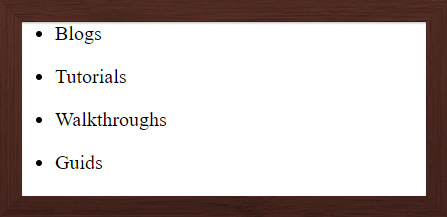
\includegraphics[width=\linewidth]{Images/Test.jpg}
        \caption{Vstup}
        \label{fig:Test}
\end{subfigure}

\begin{subfigure}{\linewidth}
        \centering
        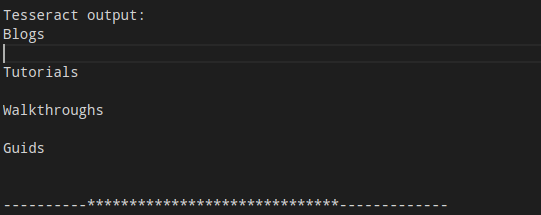
\includegraphics[width=\linewidth]{Images/Tesseract_Test.png}
        \caption{Výstup Tesseract}
        \label{fig:Tesseract_Test}
\end{subfigure}

\begin{subfigure}{\linewidth}
        \centering
        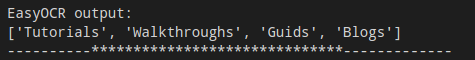
\includegraphics[width=\linewidth]{Images/easyOCR_Test.png}
        \caption{Výstup EasyOCR}
        \label{fig:easyOCR_Test}
\end{subfigure}

\begin{subfigure}{\linewidth}
        \centering
        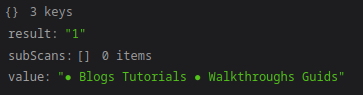
\includegraphics[width=\linewidth]{Images/penToPrint_Test.png}
        \caption{Výstup Pen to Print}
        \label{fig:penToPrint_Test}
\end{subfigure}
\caption{Základní testovací obrázek}

\end{figure}

\paragraph{Vysvětlení obrázku 1}
Z obrázku 1 je jasné, že všechna řešení byla schopna extrahovat text ze vstupního testovacího obrázku (a), je však vidět, že výstupy se od sebe značně liší a u EasyOCR také došlo k přehození slov. Nic z toho však nevzbuzovalo dojem, že nemá cenu pokračovat.


\subsection{výstupy pro reálná data}

\begin{figure}{\linewidth}
        \centering
        \includegraphics[width=\linewidth]{Images/page1.jpg}
        \caption{Vstup Reálná data}
        \label{fig:Test}
\end{figure}


\begin{figure}

\begin{subfigure}{\linewidth}
        \centering
        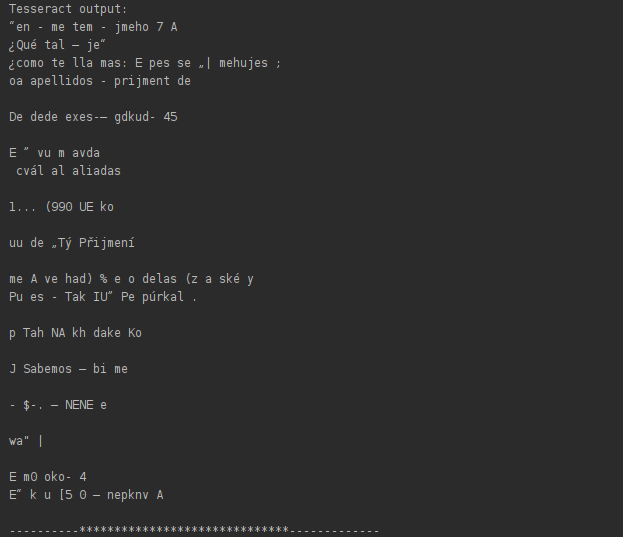
\includegraphics[width=\linewidth]{Images/Tesseract_Page1.png}
        \caption{Výstup Tesseract}
        \label{fig:Tesseract_Test}
\end{subfigure}

\begin{subfigure}{\linewidth}
        \centering
        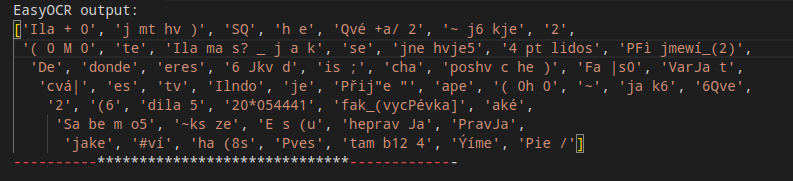
\includegraphics[width=\linewidth]{Images/easyOCR_Page1.png}
        \caption{Výstup EasyOCR}
        \label{fig:easyOCR_Test}
\end{subfigure}

\begin{subfigure}{\linewidth}
        \centering
        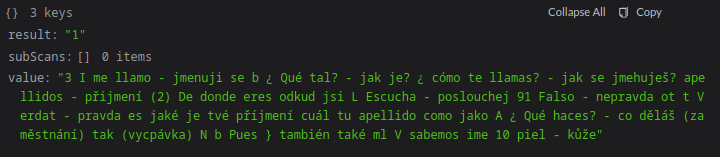
\includegraphics[width=\linewidth]{Images/penToPrint_RealDataAdjusted.png}
        \caption{Výstup Pen to Print}
        \label{fig:penToPrint_Test}
\end{subfigure}
\caption{Reálná data}

\end{figure}

\paragraph{Vysvětlení obrázku 2}
Obrázek 2 ukazuje reálný use-case, 1 stránku ze zápisků ve slovníku.
Je zde vidět klasický formát \textit{španělské slovo} - \textit{české slovo}.
Také jsou vidět klasické chyby, které mohou při zapisování slov nastat, za účelem zjištění, jak na ně budou jednotlivá \ac{OCR} řešení reagovat.

\paragraph{Vysvětlení obrázku 3}
Obrázek 3 ukazuje výstup z jednotlivých řešení.
Je nutné poznamenat, že výstup z EasyOCR byl upraven, původní výstup je jeden dlouhý řádek, pro účely tohoto textu byl řádek rozdělen.
již na první pohled je jasné, že výstup z Tesseractu ani EasyOCR není použitelný.
Ani zdaleka se tento výstup nepodobá vstupním datům, objevují se dokonce znaky které v původním textu ani neexistují.
Komerční Pen to Print si poradil podstatně lépe, ale až se zmenšeným obrázkem, původní byl na \ac{API} moc velký.
Pro srovnání byl tento upravený obrázek poskytnut i ostatním řešením, nevedlo to však k očividné změně.
Pokud se na Pen to Print výstup podíváme z blízka, je i zde možné najít hned několik odlišností od vstupního textu.
Zdá se, že problémy dělali především pomlčky a vázání sešitu.

\subsection{výstup pro testovací úryvek dat}

\begin{figure}

\begin{subfigure}{\linewidth}
        \centering
        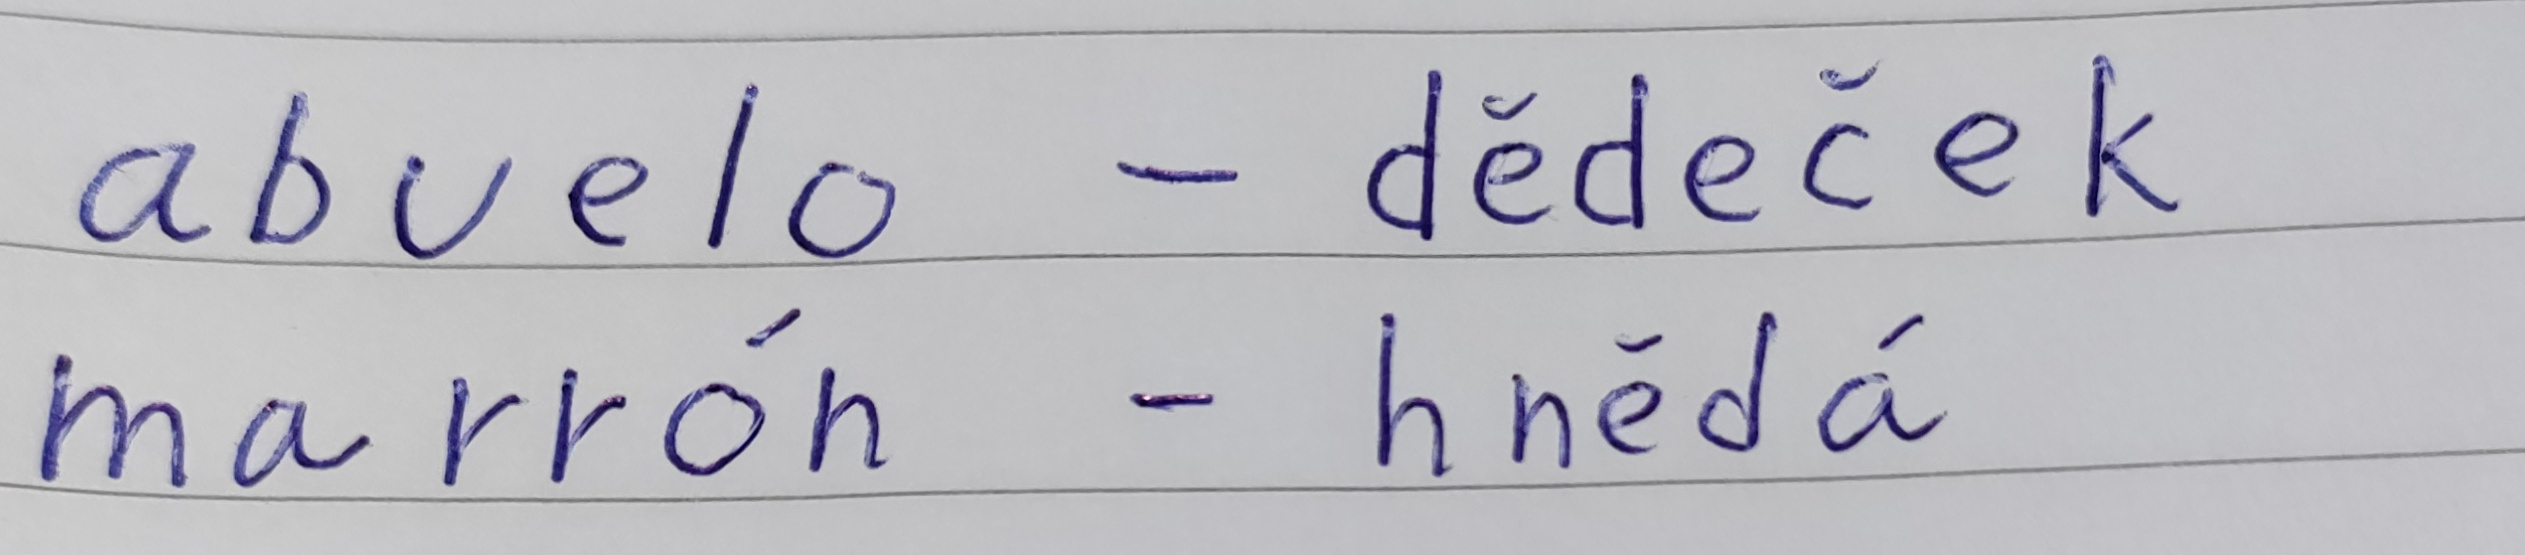
\includegraphics[width=\linewidth]{Images/pageSnippet.jpg}
        \caption{Vstup}
        \label{fig:Test}
\end{subfigure}

\begin{subfigure}{\linewidth}
        \centering
        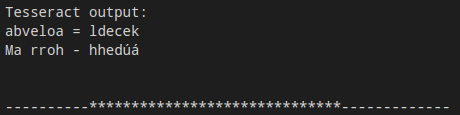
\includegraphics[width=\linewidth]{Images/Tesseract_PageSnippet.png}
        \caption{Výstup Tesseract}
        \label{fig:Tesseract_Test}
\end{subfigure}

\begin{subfigure}{\linewidth}
        \centering
        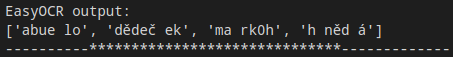
\includegraphics[width=\linewidth]{Images/easyOCR_PageSnippet.png}
        \caption{Výstup EasyOCR}
        \label{fig:easyOCR_Test}
\end{subfigure}

\begin{subfigure}{\linewidth}
        \centering
        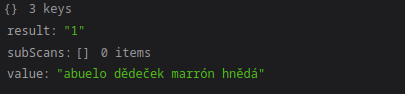
\includegraphics[width=\linewidth]{Images/penToPrint_PageSnippet.png}
        \caption{Výstup Pen to Print}
        \label{fig:penToPrint_Test}
\end{subfigure}
\caption{Malý úryvek reálných dat}

\end{figure}

\paragraph{Vysvětlení obrázku 4}
Na obrázku 4 můžeme vidět jistou kombinaci 2 předchozích testů.
Nachází se zde velice jednoduchá skutečná data v požadovaném formátu, je to však pouze malé množství dat.
Cílem bylo testovat, zda alespoň takto jednoduchá data je možné správně zpracovat.
Ani zde však není možné považovat jakékoli řešení za ideální.
Řešení využívající Tesseract má na výstupu nová slova, která se jen vzdáleně podobají vstupnímu textu.
EasyOCR řešení, při pominutí mezer navíc, správně digitalizovalo první slovo,  druhé je však k nerozeznání.
V komerčním řešení Pen to Print opět chybí pomlčky, jinak je však nejblíže požadovanému výstupu.


\section{CONCLUSIONS / ZÁVĚRY}
\subsection{závěr}
Jak je z předchozího textu jasné, nepodařilo se vytvořit nový přístup k řešení problému.
Hlavním úskalím je složitost digitalizace ručně psaného textu.
Samotná digitalizace je složitá úloha, napomáhá však standardizace jednotlivých fontů písma.
Pokud jednou naučíme rozeznávací mechanizmus určitý font rozeznávat, dále již nezáleží kdo daný font využívá, vždy je možné písmo rozpoznat.
Psaný text je však jedinečný, ani stejný znak není stejným člověkem vždy napsán stejně.
Složitost úlohy naučit rozeznávací algoritmus rozeznávat písmo i jen pro specifickou osobu je značná.
Za předpokladu úspěšnosti je pak nutné zkoumat, jak úspěšný by byl již vytvořený systém pro další osoby.
Z průzkumu trhu je vidět, že o tuto problematiku je zájem, bohužel množství prostředků které tento výzkum vyžaduje je značné, což dosti omezuje možnosti vstupu do tohoto výzkumu.
Nelze tedy než konstatovat, že ještě nějaký čas potrvá než v této práci zkoumaný use-case bude připraven i pro běžné vývojáře.
Naději dává prohlášení EasyOCR o budoucím rozšíření v tomto směru a také práce Google inženýrů na proprietárním Google vision.



% seznam zdrojů
\printbibliography

%  seznam zkratek
\printacronyms


% that's all folks
\end{document}
